% 图 17.2 —— **手写重建版**（推翻原「描摹稿」；用户 2026-10-08 裁定）
%
% 内容 = 外矩形 X + 一个**光滑闭合自由曲线**围出的 U 形舌状区（内部白）
%        + 正方形 Y（白底）+ 小方块 A（**花的**，在 U 之外）+ 标签 U Y A X。
%
% ★ 叠放（沿用 17.1 定下的手法：**画全 + 白底盖**，轮廓一律在最上层）：
%     ① 外框满铺阴影  ② U 舌形白底盖上（⇒ U 内白）  ③ Y 正方形白底盖上（⇒ Y 内白）
%     ④ A 只画轮廓（它的内部是阴影 ⇒ **花的**，用户 2026-10-08 确认）
%     ⑤ 全轮廓最上层   ⑥ 标签 U、A 加白底（两者都在阴影里；Y 在白区内不需要）
%
% 几何**实测**自 `images/17.2.png`（与本画布 1:1）：
%   外矩形 x[6.5, 532.5] y[15.5, 355.0]
%   Y 方块 x[132.5, 340.0] y[86.0, 243.0]      ← 与 A 共享底边
%   A 方块 x[257.0, 340.0] y[157.0, 243.0]
%   U 舌形边界：用墨迹密度图（近白区）逐行取左右端得到，见下方坐标表
%
% ★ 曲线做法（SOP §3.5 红线二的**退回方案**）：**手工给结点 + 一条 `smooth cycle`**，
%   **不靠拟合算法吐控制点**（那会生成噪声）。结点是量出来的，不是拟出来的。
%
% 线宽：轮廓与阴影线各一档（原描摹稿 12 档）。
\documentclass[12pt]{standalone}
\usepackage{fontspec}
\setsansfont{Arial}
\newfontfamily\mfallback{DejaVu Sans}
\usepackage{tikz}
\usetikzlibrary{patterns}

\pgfdeclarepatternformonly{hatch45}
  {\pgfqpoint{-18.385pt}{-18.385pt}}
  {\pgfqpoint{18.385pt}{18.385pt}}
  {\pgfqpoint{18.385pt}{18.385pt}}
  {\pgfsetlinewidth{3.3pt}\pgfsetstrokecolor{black}%
   \pgfpathmoveto{\pgfqpoint{0pt}{0pt}}%
   \pgfpathlineto{\pgfqpoint{18.385pt}{18.385pt}}%
   \pgfusepath{stroke}}

\def\wEdge{5.0}

\begin{document}
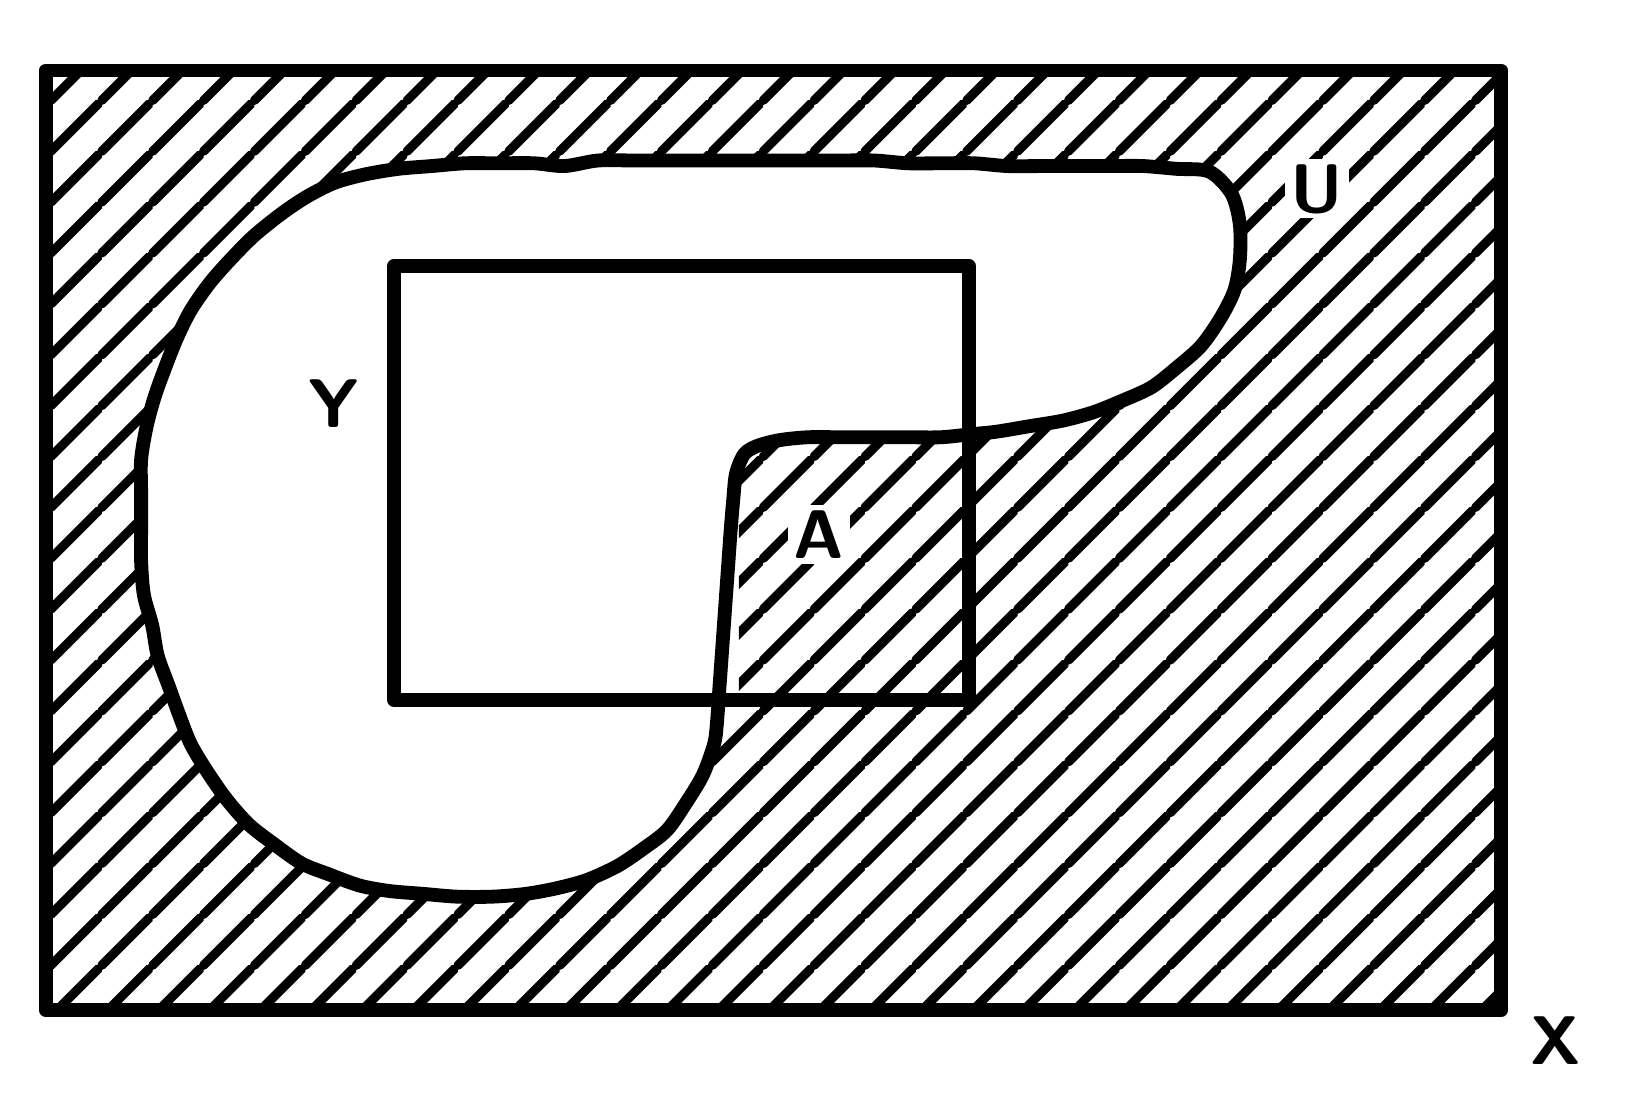
\begin{tikzpicture}[x=1pt, y=-1pt, line width=\wEdge, line cap=round, line join=round]

  %% ════ 几何 ════
  \def\Xa{6.5}   \def\Xb{532.5} \def\Ya{15.5}  \def\Yb{355.0}   % 外矩形
  \def\Pa{132.5} \def\Pb{340.0} \def\Qa{86.0}  \def\Qb{243.0}   % Y 方块
  \def\Ra{257.0} \def\Rb{340.0} \def\Sa{157.0} \def\Sb{243.0}   % A 方块

  %% U 舌形边界（实测结点，顺时针）—— 由**主连通域逐行端值**量得（已排除 Y 方块与 U 标签白底）
  %% 右侧 y=147~243 那段被 Y 方块盖住（书里也盖着）⇒ 按平滑过渡补 (400,128)(340,150)(270,190)
  \def\Ublob{(206,48) (194,50) (183,49) (170,49) (158,49) (146,50) (134,51) (122,53)
             (111,56) (101,61) (92,67) (82,75) (74,83) (66,92) (59,102) (54,112)
             (50,122) (46,133) (43,144) (41,156) (41,168) (41,180) (41,193) (42,205)
             (45,216) (47,227) (51,238) (55,249) (59,259) (65,269) (72,279) (80,288)
             (89,295) (99,302) (109,306) (120,310) (131,312) (143,313) (155,314)
             (168,314) (180,313) (191,311) (202,308) (213,303) (222,297) (231,290)
             (238,280) (244,270) (248,259) (249,252) (250,238) (251,224) (252,210)
             (253,196) (254,182) (255,170) (256,161) (259,154) (264,151) (272,149)
             (282,148) (294,148) (306,148) (318,148) (330,148) (340,147) (350,146)
             (362,144) (374,142) (385,139) (395,135) (406,130) (415,123) (424,115)
             (431,105) (436,95) (438,84) (438,71) (435,60) (427,52) (415,51) (403,50)
             (391,50) (379,50) (367,50) (354,50) (342,49) (330,49) (318,49) (306,48)
             (293,48) (281,48) (269,48) (256,48) (244,48) (232,48) (219,48)}

  %% ① 满铺阴影
  \begin{scope}
    \clip (\Xa,\Ya) rectangle (\Xb,\Yb);
    \fill[pattern=hatch45] (\Xa,\Ya) rectangle (\Xb,\Yb);
  \end{scope}

  %% ② U 舌形：白底盖上（内部变白）
  \fill[white] plot [smooth cycle] coordinates {\Ublob};

  %% ③ Y 方块：白底盖上
  \fill[white] (\Pa,\Qa) rectangle (\Pb,\Qb);

  %% ④ "A 方块"**不是独立矩形**（用户 2026-10-08 第二次更正）：
  %%    它的**上边与左边是 U 曲线自己拐出来的**（近直角、弧度小）；
  %%    **右边与底边就是 Y 方块的边**。⇒ **不许再 `\draw` 一个矩形**。
  %%    这一块整个落在 Y 之内，会被 Y 的白底盖白，而书里它是**花的** ⇒ **补铺一次阴影**。
  %%    （区域取 x[257,340] y[150,243] —— 上边对齐曲线的凹口顶）
  \fill[pattern=hatch45] (\Ra,150.0) rectangle (\Rb,\Sb);

  %% ⑤ 轮廓（**全在最上层**）：U 曲线必须在这里，因为**凹口的上边/左边在 Y 方块内部、要露出来**
  \draw (\Xa,\Ya) rectangle (\Xb,\Yb);                                   % 外框
  \draw plot [smooth cycle] coordinates {\Ublob};                        % U 舌形（含凹口）
  \draw (\Pa,\Qa) rectangle (\Pb,\Qb);                                   % Y

  %% ════ 标签（位置≈原书字形框中心；字符已核过：U Y A X 全大写）════
  \node[anchor=center,inner sep=2pt,fill=white,font=\fontsize{30.0}{37.5}\selectfont] at (466.0, 58.0) {\textsf{\textbf{\textit{U}}}};
  \node[anchor=center,inner sep=0pt,font=\fontsize{30.0}{37.5}\selectfont] at (111.0,136.0) {\textsf{\textbf{\textit{Y}}}};
  \node[anchor=center,inner sep=2pt,fill=white,font=\fontsize{30.0}{37.5}\selectfont] at (286.0,183.0) {\textsf{\textbf{\textit{A}}}};
  \node[anchor=center,inner sep=0pt,font=\fontsize{33.0}{41.2}\selectfont] at (552.0,366.0) {\textsf{\textbf{\textit{X}}}};

  \pgfresetboundingbox
  \path[use as bounding box] (0,0) rectangle (569,384);
\end{tikzpicture}
\end{document}
